\chapter{緒論}
\label{chapter:intro}

\section{背景與動機}

在人工智慧的浪潮下, 已有愈來愈多工廠只餘機器人在工作, 人們只需定期去工廠檢
查確保正常營運。科技技術的進步往往能便利人們的生活,也漸漸改變人們生活的方
式, 以日常生活舉例, 當需要購買生活用品時會去便利超商、量販店或是直接由網路購
物商城購買商品, 最近更出現了不須服務人員的無人商店, 如: 位於西雅圖的 AmazonGo
無人商店, 主打顧客挑選商品完就可以帶著商品離開, 不須交由店員結帳付款, 而是自動
辨識顧客挑選的商品進行信用卡扣款, 省去了等待排隊的時間; 而網路購物也是相當便
利, 由廠商針對顧客網路訂單從倉儲進行集貨並由貨運公司進行運輸到客戶手中,其中
許多廠商為了提高集貨的效率已經著手於倉儲的自動化。然而在無人商店跟倉庫的應
用中,現今還無法達成實質無人化,原因是因為如無人商店內商品上架仍需人去逐一
整齊擺放,而倉庫在進行商品分類與打包時也須有人去掃描商品條碼才可以知道商品
代號和該怎麼打包。這些自動化任務成了現在業界都想解決的問題。


而亞馬遜揀取挑戰Amazon Picking Challenge,便因此而生。在自動化的亞馬遜公司倉庫中,成千上萬的移動機器人將1平方公尺的貨架單元從存儲位置移動到揀選區,然後再移回存儲位置。工人須站在揀選區,從貨架上挑選物品,並將它們放入運往客戶的箱子中。貨架上的典型箱中最多可包含10個物品 - 通常緊密堆積在一起 , 員工可以識別正確的產品,從箱子中取出,掃描條形碼進行驗證,然後放置物品在一個盒子裡,所有這些都只需幾秒鐘。典型的亞馬遜倉庫擁有數百萬種不同的產品。雖然許多這些物品形狀簡單,如書籍和DVD,但也有如泰迪熊,兒童項鍊,真空包裝的USB棒,這些不規則的其他形狀、物品。在這過程中目前仍無法省略的便是人工揀取物品放置箱子的流程。因此亞馬遜公司認為自動化揀取是機器人操作中一個相當重要的技術,並且將可應用於許多領域上如倉庫、大量製作、服務機器人(service robotics)上。為了自動化這個任務,亞馬遜公司連續3年舉辦亞馬遜揀取競賽,並祭出高額獎金,邀請機器人名校來解決自動化夾取問題。由此可知自動化夾取問題的重要性。


然而除了自動化夾取任務外,放置也是相當重要的議題,如上述所提無人商店上架,除了將商品揀取放上架子外,還要確保架上的商品是否有擺正,也就是商品商標或是品牌文字是否有朝外。而在倉庫中生產線分類物品時,也須將物品夾取並放置到輸送帶上,並確保條型碼朝上,以便掃描機能掃描條碼進行分類。這兩者任務雖有所不同,但皆可歸類為需針對商品上語意標籤如品牌文字或條碼去進行套定姿態擺放任務。結合語意標籤進行特定姿勢擺放任務是一
較新穎之領域, 相當具有挑戰性。便可實際應用於倉庫與無人商店,將可降低大量人力
與時間成本。


\section{目標與貢獻}

\subsection{問題定義}
過去已有許多研究去解決雜亂環境中夾取的問題,再亞馬遜揀取挑戰中,許多新穎的方法也被創造出來,並具有很好的效果,
但是卻鮮少有人去接觸放置的問題。在無人商店與倉庫的許多應用中,夾取與放置任務都十分重要,如無人商店上架必
須放置商品時,品牌文字或商標需朝外放。放置任務尤其以特定姿態放置任務最為困
難,因為其牽涉到物品姿態以及夾取可行性。如何設計一個考慮到物品姿態以及夾取可行性的系統是本研究的主要議題。
以往考慮到姿態夾取的研究~\cite{zeng2016multi}以物體幾何模型為考量,但卻未考量到幾何模型對稱的問題。
因此,在此研究中, 將設計特別的標注規則去定義物品姿態並創建資料庫:物品表面的一小部分作為語意標籤, 此語意標籤不僅可以作為物品三維姿態辨識的依據, 更可以做為操作行
為的依據, 物品上可能有不只一個語意標籤如品牌文字、條形碼等, 本研究將專注於在雜亂環境中,以品牌文字為線索進行特定姿勢放置任務。

\subsection{挑戰}
\begin{itemize}
\item 以往定義物品姿態,皆是由三維模型來定義,但是卻不適用於形狀對稱的物體,因為物品的表面語意如品牌文字、條碼並不會反應在三維模型中,因此得從圖片下手,要如何以2維圖片去定義物體的3維姿態,是此研究的重要議題。
\item 在雜亂的環境中,產品物件可能互相堆疊,造成物品部分或全部遮蔽 (occlusion)。
由於品牌文字可能只在產品物件的特定平面位置, 也可能在初始位置即被遮蔽,如何偵測品牌文字或是藉由主動式操作系統改變環境場景,找出品牌文字所在的一面,是本研究重要目標之一
\item 受限於機器手臂與末端效應器(End effector)的工作範圍,即使預測出物體姿態,特定姿態夾取與放置行為仍可能無法執行,或是在移動過程中會遇到障礙物,造成任務失敗。因此如何透過夾爪的設計與機器人操作系統的架設,讓物體容易夾取,也是本研究的重要議題之一。
\end{itemize}

\subsection{論文貢獻}
\begin{itemize}
\item \textbf{主動式操作搭配雙手臂協作} 除卻被動利用物件辨識與姿態辨識的結果,本論文運用主動式操作概念去改變雜亂場景,去達到對單一物品與品牌文字最佳的的感知能力。本論文提出的方法不僅可以改變相機視角去看到最少遮蔽的品牌文字,也使用雙手臂協作的方式去操作商品,以達到最佳的放置成效。
\item \textbf{建立基準商品語意資料集以訓練與測試模型與演算法效果} 在現今的影像物件分割技術下,訓練一個深度卷積神經網路需要數量龐大且有標注的資料集。
為了訓練物件切割模型,本論文建立了一個資料集,此資料集包含20個物件,且每個物件都有條碼與品牌文字。此資料集包含來自真實世界與虛擬環境的訓練資料以及真實環境的測試集用來評估放置任務的成效。
\end{itemize}

\section{論文架構}
本論文架構總共有五個章節。第一章為緒論,包含背景動機、以及目標貢獻。第二章則介紹文獻回顧,包含Amazon Picking Challenge競賽回顧、主動式視覺與主動式操作系統、物品夾取可行性預測、雙手臂機械協作、機器人操作領域之基準訓練測試集,快速瀏覽在與本論文相關之研究領域,第三章則為系統架構與方法,依序介紹系統的硬體架構與工作環境、商品語意資料庫、基於品牌文字之夾取可行性預測、主動式操作系統。第四章介紹本研究的兩大實驗:品牌文字切割評估、主動式操作系統評估。最後一章為本論文的結論與未來展望。

\begin{figure}[H]
	\centering
	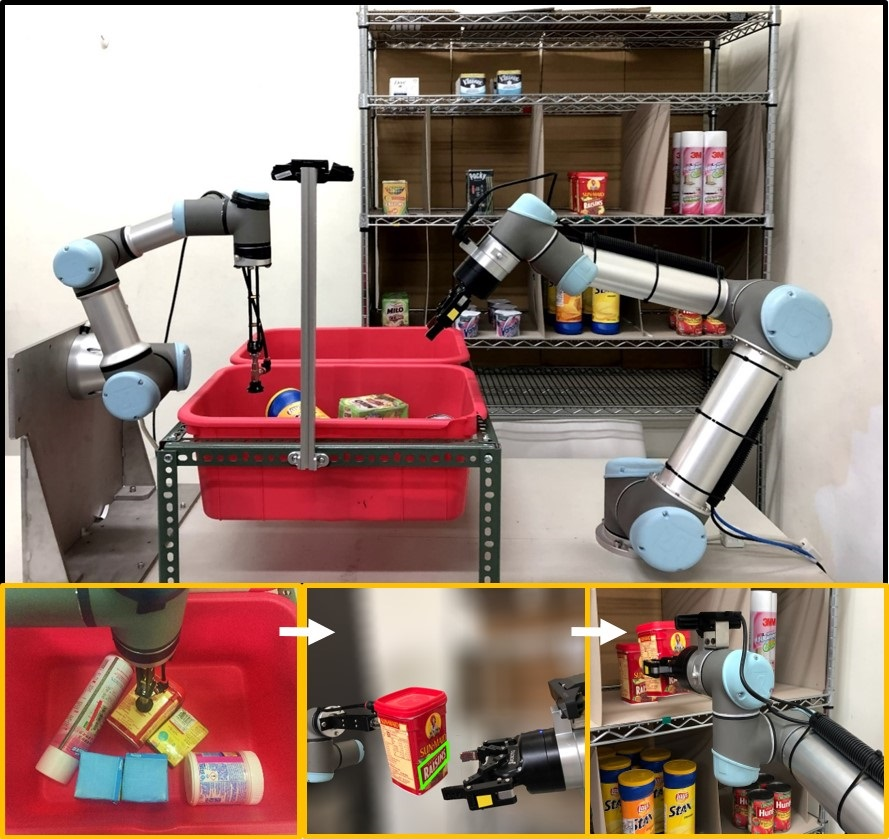
\includegraphics[height=!, width=1.0\linewidth, keepaspectratio=true]
	{./figures/pose-aware-placing-teaser-v3.jpg}
  \caption{本論文利用商品文字(商品上的其中一個語意標籤)作為特殊姿態放置的依據,並設計雙手臂協做的主動式操作系統去解決物品遮蔽的問題。圖左下到右下:吸盤式夾爪透過物品或品牌文字語意線索去夾取物品至空曠空間,而兩指式夾爪再透過品牌文字線索去執行放置任務。}
  \label{figure:teaser}
\end{figure}
